% ===================================================================
% SECTION 3: METHODOLOGY
% ===================================================================
\section{Methodology}

% --- Subsection 3.1: Algorithms ---
\subsection{Algorithms}

% --- Slide 1: From Dynamic Programming to Reinforcement Learning ---
\begin{frame}
    \frametitle{From Dynamic Programming (DP) to Reinforcement Learning (RL)}

    % --- TOP PART: Side-by-side equations ---
    \begin{columns}[T]
        \begin{column}{0.5\textwidth}
            \begin{block}{1. Dynamic Programming Recurrence for KP}
                State value is the maximum value by:
                \begin{itemize}
                    \item \textbf{Skip item $i$:} Value is the future reward from the remaining state, $V(i-1, w)$.
                    \item \textbf{Take item $i$:} Value is the immediate reward $v_i$ + future reward from the new state, $V(i-1, w-w_i)$.
                \end{itemize}
                
                \begin{align*}
                    V(i, w) = 
                    \begin{cases}
                        V(i-1, w) & \text{if } w_i > w \\
                        \max( V(i-1, w), \\
                        v_i + V(i-1, w-w_i) ) & \text{if } w_i \le w
                    \end{cases}
                \end{align*}
            \end{block}
        \end{column}

        \begin{column}{0.5\textwidth}
            \begin{block}{2. The Bellman Equation (Element-wise)}
                State value is the expected immediate reward plus the discounted expected future reward.
                \begin{align*}
                    V_{\pi}(s) = \sum_{a \in A} \pi(a|s) \bigg[ & \sum_{r \in R} p(r|s, a)r \\
                                                            & + \gamma \sum_{s' \in S} p(s'|s, a)V_{\pi}(s') \bigg]
                \end{align*}
                % \begin{itemsize}
                %     \item $V_{\pi}(s)$ is the value of state $s$ under policy $\pi$.
                %     \item $\pi(a|s)$ is the probability of taking action $a$ in state $s$.
                %     \item $p(r|s, a)$ is the probability of receiving reward $r$ after taking action $a$ in state $s$.
                %     \item $\gamma$ is the discount factor for future rewards.
                % \end{itemsize}
                \begin{itemize}
                    \item \textbf{DP} recurrence is a specific, deterministic instance of the Bellman equation.
                \end{itemize}
            \end{block}
        \end{column}
    \end{columns}
    
    % --- BOTTOM PART: RL Definitions ---
    \begin{alertblock}{Modeling KP as an RL Problem}
        \begin{itemize}
            \item \textbf{State ($s_t$):} The set of available items and the current remaining knapsack capacity.
            \item \textbf{Action ($a_t$):} The selection of one item from the available set.
            \item \textbf{Reward ($R_{t+1}$):} The value ($v_i$) of the selected item.
            \item \textbf{Policy ($\pi_\theta(a|s)$):} A neural network mapping states to action probabilities.
            % \item \textbf{Episode ($\tau$):} A sequence of item selections until a terminal state.
        \end{itemize}
    \end{alertblock}

\end{frame}

% --- Slide 2: From Bellman to PPO: An Evolutionary Path ---
\begin{frame}
    \frametitle{From Bellman to PPO: An Evolutionary Path}
    \small % Use smaller font to fit content

    % Two-column layout for formulas
    \begin{multicols}{2}
        \begin{enumerate}
            \item \textbf{Bellman Equation}
            \[ V^\pi(s) = \mathbb{E}[r + \gamma V^\pi(s')] \]

            \item \textbf{Value Function Approx.}
            \[ V_\phi(s) \approx V^\pi(s) \]

            \item \textbf{REINFORCE (Policy Gradient)}
            \[ \nabla_\theta J = \mathbb{E}\left[\nabla_\theta \log \pi_\theta(a|s) \cdot G_t\right] \]
            
            \columnbreak % <--- Force a column break here

            \item \textbf{A2C (Actor-Critic)}
            \[ \nabla_\theta J \propto \sum_t \nabla_\theta \log \pi_\theta(a_t|s_t) \cdot \hat{A}_t \]
            \textit{($\hat{A}_t = r + \gamma V_\phi(s') - V_\phi(s)$: TD-based)}

            \item \textbf{PPO (Clipped Objective)}
            \[ \mathcal{L}^{\text{CLIP}}(\theta) = \mathbb{E}\left[\min\left(r_t \hat{A}_t,\ \text{clip}(r_t, 1\pm\epsilon) \hat{A}_t\right)\right] \]
            where \( r_t = \dfrac{\pi_\theta(a_t|s_t)}{\pi_{\theta_{\text{old}}}(a_t|s_t)} \)
        \end{enumerate}
    \end{multicols}
    \vspace{-1em} % Add some space between the equations and the text below
    % Evolutionary Path with clear explanation
    \begin{block}{The Evolutionary Path to PPO}
        \begin{description}
            \item[Bellman $\to$ Value Approx.] Replace exact $V^\pi$ with a learnable $V_\phi(s)$ (e.g., neural net). Enables scalability to large or continuous state spaces.

            \item[Value Approx. $\to$ REINFORCE] Shift from value-based to direct policy optimization. More suitable for stochastic or complex action spaces.

            \item[REINFORCE $\to$ A2C] Replace Monte Carlo return $G_t$ with TD-based advantage $\hat{A}_t$. Reduces variance, enables online updates, and improves sample efficiency.

            \item[A2C $\to$ PPO] Replace policy gradient with clipped surrogate objective. Prevents destructive updates and stabilizes training.
        \end{description}
    \end{block}
\end{frame}

% --- Slide 3: PPO Algorithm and Model Architecture ---
\begin{frame}
    \frametitle{PPO: Algorithm and Architecture}

    \begin{columns}[T]
        \vspace{-1em}
        
        % --- LEFT COLUMN: PPO Algorithm Flowchart ---
        \begin{column}{0.5\textwidth}
            \begin{block}{Training Algorithm}
                \begin{figure}
                    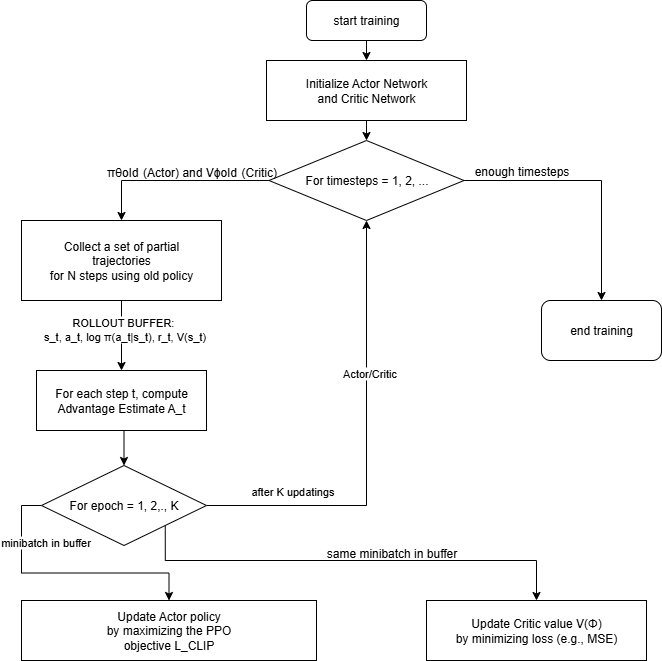
\includegraphics[width=0.85\textwidth, height=0.63\textheight]{PPO_training_manual.png}
                    \caption{The PPO training loop using an Actor-Critic framework.}
                \end{figure}
                \vspace{-1.5em}
                \begin{itemize}
                    \item Multiple optimization on the same minibatch.
                \end{itemize}
            \end{block}
        \end{column}

        % --- RIGHT COLUMN: PPO Model Architecture ---
        \begin{column}{0.5\textwidth}
            \begin{block}{Model Architecture}
                \begin{figure}
                    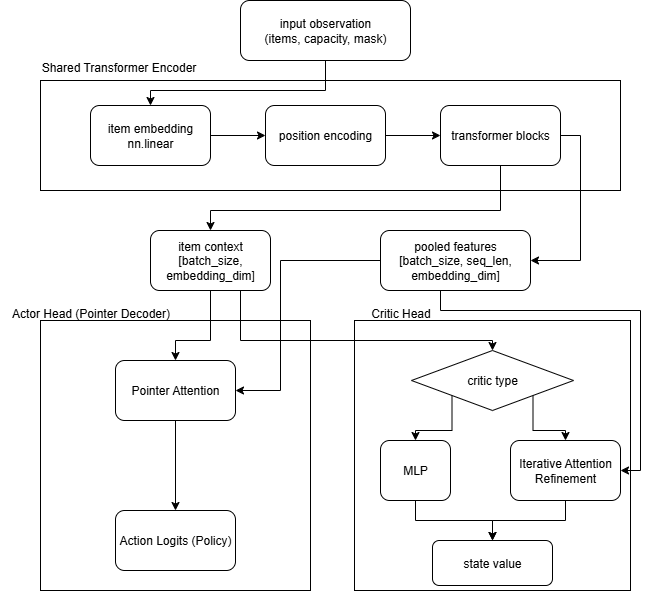
\includegraphics[width=0.85\textwidth, height=0.6\textheight]{ppo_model_manual.png}
                    \caption{The model has two heads: one for the policy (Actor) and one for the value (Critic).}
                \end{figure}
                \vspace{-1.5em}
                \begin{itemize}
                    \item Actor and Critic share the same encoder.
                    % \item The Actor outputs a probability distribution over actions (items).
                    % \item The Critic outputs a value estimate for the current state.
                \end{itemize}
            \end{block}
        \end{column}

    \end{columns}
\end{frame}

